% Adapted from Figure 3 in the arXiv source of Gluchowski--Menz,
% arXiv:2508.08459v1, main.tex (https://arxiv.org/src/2508.08459v1).
% Retains the paired unit squares, axes, ticks and gray/red palette.
% Uses positive slices and exact intersections; blue is the added region.
% Coordinates: x=p_{1|10}, y=p_{1|01}, z=p_{1|00}, with p_{1|11}=0.
% Earlier gray: x<1/2 or x<y+z or y<=z.
% Earlier red: max(y,z)<sqrt(2)*(1-x), outside gray.
% New blue: z<=y*(1-x), outside gray and red.
% The polygon formulas below are used only for z=1/100 and z=1/10.
\begingroup
\color{black}
\begin{tikzpicture}[scale=4, line cap=round, line join=round]
  \foreach \z/\shift/\denom in {0.01/0/100,0.1/1.55/10} {
    \begin{scope}[xshift=\shift cm]
      \pgfmathsetmacro{\oldcross}{(sqrt(2)+\z)/(1+sqrt(2))}
      \pgfmathsetmacro{\redend}{1-\z/sqrt(2)}
      \pgfmathsetmacro{\newcross}{1-sqrt(\z/sqrt(2))}
      \pgfmathsetmacro{\newend}{(1+\z+sqrt(1-6*\z+\z*\z))/2}

      % Regions in the earlier figure, with rounded vertices replaced
      % by their exact expressions.
      \fill[gray!25] (0,0) -- (1,0) -- (1,\z) -- (0.5,\z)
        -- (0.5,{0.5-\z}) -- (1,{1-\z})
        -- (1,1) -- (0,1) -- cycle;
      \fill[red!25] (0.5,\z) -- (\redend,\z)
        -- (\oldcross,{\oldcross-\z})
        -- (0.5,{0.5-\z}) -- cycle;

      % Additional coverage: above both y=sqrt(2)*(1-x) and
      % y=z/(1-x), and below y=x-z.
      \fill[blue!25] (\oldcross,{\oldcross-\z})
        -- (\newend,{\newend-\z})
        -- plot[domain=\newend:\newcross,samples=100,variable=\x]
          ({\x},{\z/(1-\x)}) -- cycle;

      % Boundaries between the regions. The blue curve is the new
      % criterion's boundary outside the previously shaded regions.
      \draw[thick] (0.5,\z) -- (0.5,{0.5-\z}) -- (1,{1-\z});
      \draw[thick] (0.5,\z) -- (1,\z);
      \draw[thick,dashed,red!70!black]
        (\oldcross,{\oldcross-\z}) -- (\redend,\z);
      \draw[thick,blue!70!black]
        plot[domain=\newcross:\newend,samples=100,variable=\x]
          ({\x},{\z/(1-\x)});

      % Axes and ticks follow the source figure.
      \draw (0,0) rectangle (1,1);
      \draw[->] (-0.02,0) -- (1.08,0)
        node[below right] {$p_{1\mid10}$};
      \draw[->] (0,-0.02) -- (0,1.08)
        node[above left] {$p_{1\mid01}$};
      \foreach \t in {0,1} {
        \draw (\t,0) -- (\t,-0.02) node[below] {\small $\t$};
        \draw (0,\t) -- (-0.02,\t) node[left] {\small $\t$};
      }
      \draw (0.5,0) -- (0.5,-0.02) node[below] {\small $\tfrac12$};
      \draw (0,0.5) -- (-0.02,0.5) node[left] {\small $\tfrac12$};
      \node at (0.5,-0.20) {$p_{1\mid00}=\tfrac1{\denom}$};
    \end{scope}
  }
  % Shared legend; white is deliberately described only relative
  % to the displayed criteria, not as a claim of nonergodicity.
  \begin{scope}[shift={(0.12,-0.42)},every node/.style={anchor=west,font=\small}]
    \fill[gray!25] (0,0) rectangle (0.065,0.055);
    \node at (0.09,0.0275) {Time-scaling criteria (2025)};
    \fill[red!25] (0,-0.11) rectangle (0.065,-0.055);
    \node at (0.09,-0.0825) {Long-lived-state criterion (2026)};
    \fill[blue!25] (1.40,0) rectangle (1.465,0.055);
    \node at (1.49,0.0275) {Added by orientability};
    \draw (1.40,-0.11) rectangle (1.465,-0.055);
    \node at (1.49,-0.0825) {Not covered by these criteria};
  \end{scope}
\end{tikzpicture}
\endgroup
